\documentclass[12pt, a4paper]{article}
\usepackage[T1]{fontenc}
\usepackage[utf8]{inputenc}
\usepackage{lmodern}
\usepackage{microtype}
\usepackage{amsmath, amssymb}
\usepackage{booktabs}
\usepackage{graphicx}
\usepackage{caption}
\usepackage[style=authoryear, backend=biber]{biblatex}
\addbibresource{references.bib}
\usepackage[margin=2.5cm]{geometry}
\usepackage{setspace}
\usepackage{xcolor}
\usepackage{hyperref}
\usepackage{threeparttable}

\onehalfspacing

\newcommand{\todo}[1]{\textcolor{red}{\textbf{[TODO: #1]}}}
\newtheorem{proposition}{Proposition}
\newcommand{\rr}{\mathbf{r}}

\title{Reinstatement out of equilibrium: shock speed and the destination of new work}
\author{Joakim Storck}
\date{Draft: \today}

\begin{document}
\maketitle

\begin{abstract}
\noindent
Storck (2026) closes the spatial task-based model as a static
equilibrium and reads its consequences as comparative statics between
two rest points. This paper turns the same model into laws of motion and
asks what the static account cannot: how the transition unfolds in time,
and how its outcome depends on the speed of the shock. The technology matures gradually --- a
logistic diffusion over a calendar window --- so that displacement, and
the new tasks it seeds on the boundary of the technology field, are
released as a flow rather than at once. The single new object the
dynamics require is a stock of \emph{unbound} task mass: the seeded work
that has been created but not yet attached to any occupation, the third
fate of new tasks that the static model creates and discards at every
evaluation. Its trajectory $U(t)$ is the transitional mismatch between
destruction and creation, and it is the model's central dynamic
observable. Binding draws this stock down: new work is attracted to the
occupations whose held capabilities best match it, but each occupation
can absorb only at a rate limited by its size, so a saturated best match
leaves a residue that cascades to the next-best match. The outcome is
governed by a single ratio, the tempo of the shock against the tempo of
redistribution. When redistribution keeps pace, reinstated work is bound
by the high-skill specialists whose capabilities fit the frontier; when
the shock outruns redistribution, small best-matched occupations cannot
absorb it and the mass is taken instead by the large, lower-skilled
occupations that can, a forced downgrading. The same technology and the
same field thus yield materially different distributions of work
depending only on the tempo: the final allocations of the slow and fast
regimes correlate at $0.37$. The two regimes are the proved limits of
the binding law, and the destination moves monotonically between them
with the tempo. This path-dependence of the destination is invisible to the
equilibrium framework, whose fixed point sees only the endpoint. The
realisation is illustrative, inheriting the calibration of Storck
(2026).
\end{abstract}

\tableofcontents
\newpage

%% ============================================================
\section{Introduction}
\label{sec:intro}
%% ============================================================

A technological breakthrough can happen overnight. Its consequences
take years to unfold, and while they do, the labour market is already
responding. Firms invest, new work practices spread, training
programmes equip engineers and workers with the skills the technology
demands, and schools carry the new knowledge to the next cohort. As the
technology diffuses and matures it displaces old tasks and introduces
new ones. Some workers find new work where they stand, others move to
reach it. These processes run in parallel, and each runs at its own
speed.

Research has measured these speeds separately. The diffusion literature
has timed the technology since \textcite{griliches1957hybrid} fitted
logistic curves to the spread of hybrid corn. New technologies take
decades to reach their ceilings, general-purpose technologies deliver
their gains a generation after they arrive, and adoption lags differ
widely across countries \parencite{david1990dynamo,
comin2010exploration}. The mobility literature has timed the workers.
Occupational moves are slow and costly because much of human capital is
specific to tasks, and a mover loses the part that does not transfer
\parencite{kambourov2009occupational, gathmann2010}. The task-based
tradition supplies the content of the shock. Automation displaces
labour from existing tasks, the creation of new tasks reinstates it,
and the balance between the two sets the demand for labour
\parencite{acemoglu2018race, acemoglu2019automation}. Each clock has
been measured on its own. No framework runs them against each other and
asks who ends up with the new work.

The task-based framework reads the consequences of a technology as the
difference between two rest points. Its dynamics, where it has them,
belong to the technology, to which tasks are automated and when new
ones arrive, while workers reach their new allocation instantaneously
\parencite{acemoglu2019automation}. The intermediate path of the
allocation drops out, and with it the cost of the transition and any
dependence of the outcome on the speed of the shock. Yet the transition
is where the human consequences of automation are felt. The central
claim of this paper is that the speed of the shock relative to the
speed of adjustment determines not merely how costly the transition is
but \emph{who ends up doing the reinstated work}.

The framework we build on is developed in two papers.
\textcite{storck2026geometry} map tasks and occupations from O*NET
statements onto a two-dimensional disk, where each occupation is a
bundle of tasks. \textcite{storck2026fields} builds the model of
technological change on that geometry. The market price of skill varies
over the space as a directional field, and a technology arrives as a
Gaussian augmentation field. Automation removes the high-priced tasks
of a bundle. Reinstatement seeds new tasks on the gradient boundary of
the field, and they survive as human work where labour remains the
cheaper producer. That model is closed as a static equilibrium, with
the adjustment dynamics left explicitly for later work. The
rise-and-fall of employment which \textcite{bessen2019demand}
documents over time appears in it only as a cross-section over the
demand elasticity, not as a trajectory. This paper is that later
work.

We make one structural addition and otherwise reuse the static model
unchanged. That model creates new task mass on the boundary ring and
lets it meet three fates. Capital captures one part and occupations
bind another, while the unbound remainder is created and discarded at
every evaluation, with no home in the model. The dynamic model gives it
a home, a stock $U(\rr,t)$ of unbound task mass that fills as the
technology matures and drains as occupations bind it. This stock is the
only genuinely new object; population, price, displacement, seeding, and
the bundle operator are the static model's, now read as rates rather
than as a solved equilibrium. The trajectory of the stock, $U(t)$, is the
transitional mismatch between destruction and creation, and it is the
first observable the static model cannot produce.

The second, and the paper's central result, concerns binding. Unbound
work seeks the occupations whose held capabilities best match it, but
an occupation can take on new work only at a rate limited by its size,
so a small best match saturates and leaves a residue for the next-best
match. The shock seeds new work at one tempo and occupations bind it at
another, so the realised allocation depends on a race. We show that the
ratio of the two tempos governs not only the height and duration of the
transitional mismatch $U(t)$ but the final destination of the work. A
gradual shock lets the best-matched occupations keep pace, and the
high-skill specialists whose capabilities fit the frontier bind the
reinstated work. A shock that outruns redistribution forces the work
onto the large, lower-skilled occupations that can absorb it fastest, a
downgrading that the gradual transition avoids. The two regimes run
through the same technology and the same field, and their final
allocations of reinstated work correlate at $0.37$. Both endpoints are
proved as limits of the binding law. Absorption faster than the shock
converges to the match-weighted allocation and absorption slower than
the shock to initial size shares, and the realised destination moves
monotonically between the two as the tempo varies
(Section~\ref{sec:homotopy}). The destination itself is
path-dependent, and the equilibrium framework sees none of it.

That reallocation takes time and shapes equilibrium is an old
observation. In the islands tradition workers move slowly between
markets and unemployment is the reallocation in progress
\parencite{lucas1974equilibrium, alvarez2011search}; distance appears as
a cost, but there is no space in which the shock and the workers'
capabilities are located together. \textcite{csahin2014mismatch} measure
the unemployment produced when job seekers search in the wrong markets:
workers waiting for work. \textcite{guvenen2020multidimensional}
measure mismatch inside the match, as the distance between the skills an
occupation requires and those its worker brings. The unbound stock of
this paper is the reverse
object, work that has been created but not yet attached to any
occupation, mismatch upstream of any vacancy. Its hump is the model's
analogue of their cyclical index, driven by task destruction and
creation rather than by the business cycle. Closest on the question of
tempo, \textcite{adao2024fast} relate the speed of a technological
transition to skill specificity. When the benefited activities require
skills far from the rest of the economy, incumbents cannot reallocate
and demand waits for the entry of new generations. In their model the
economy converges to the endpoint the technology pins down, regardless
of the path. Here the tempo of the shock races a fixed speed of
reallocation, and the endpoint moves with it. The same technology, run
slowly or quickly through the same economy, binds the reinstated work
to different occupations. The tempo is also a policy margin.
\textcite{guerreiro2022should} find it optimal to tax robots while the
workers who cannot move remain in the labour force, and
\textcite{beraja2025inefficient} to slow automation while displaced
workers reallocate under borrowing constraints. Our result gives that
lever a second consequence: pacing moves the destination of the work.
The calibration remains illustrative in the discipline of
\textcite{storck2026fields}, and we make no causal claim from it.

%% ============================================================
\section{The static foundation}
\label{sec:foundation}
%% ============================================================

We recall only what the dynamics require. The geometry --- the disk,
its coordinates, and the mapping of tasks and occupations into it --- is
constructed and validated in \textcite{storck2026geometry}; the model
of technological change on it, and the calibration used here, are from
\textcite{storck2026fields}.

Tasks lie on the unit disk in polar coordinates $\rr = (\xi,\chi)$, with
$\xi$ a domain orientation and $\chi$ a depth. The market price of skill
is a directional field
\begin{equation}
\ln \Pi(\rr) = m_0 + m_1\cos\xi + m_2\sin\xi
+ \chi\,(m_3 + m_4\cos\xi + m_5\sin\xi),
\end{equation}
high in the socio-cognitive directions and low in the service and manual
ones \parencite{storck2026geometry}. Depth is what
\textcite{adao2024fast} call skill specificity; the
geometry gives it a direction, and the price field decides where
specificity pays. A technology is a Gaussian field
$\phi_K(\rr) = A_K\exp(-\tfrac12\lVert\rr-\mathbf p_K\rVert^2/z_K^2)$,
with maturity $A_K$, centre $\mathbf p_K$, and reach $z_K$. Capital bears
a task only where it is the cheaper producer, so the operated share is
\begin{equation}
a(\rr) = \Bigl[1+\exp\!\bigl(-\bigl(s_K\phi_K(\rr) - R/\Pi(\rr)\bigr)/\tau\bigr)\Bigr]^{-1},
\label{eq:operated}
\end{equation}
where $\tau$ is the width of the adoption margin, and the condition
crosses first where the price $\Pi$ is high: automation takes the
dearest work. Each occupation $o$ is a bundle $b_o(\rr)$ with centroid
$\mu_o$; its displaced mass is $D_o = \int b_o a$, and the aggregate
displacement is $\Delta\Gamma^D = \sum_o L_o D_o$.

Reinstatement creates new task mass $M = \gamma\,\Delta\Gamma^D$ on the
gradient ring of the field,
$\hat g(\rr) = \lVert\nabla\phi_K\rVert / \int\lVert\nabla\phi_K\rVert$,
which peaks at distance $z_K$ from the centre. A seeded task survives as
human work only where the operated share is low, through the survival
gate $(1-a)$: deep in the core, where capital dominates, the same seed is
captured by capital. The surviving seed density is therefore
$\hat g\,(1-a)$, concentrated on the boundary crescent. An occupation can
take a seeded task only where its capabilities match the task's
requirements. The implemented readiness, eq.~(attachment) of
\textcite{storck2026fields}, is symmetric and local,
\begin{equation}
e_o(\rr)
= \exp\!\bigl[-\bigl(\delta_o(\rr)
  + \lambda_{\mathrm{over}}\,\bar\delta_o(\rr)\bigr)/\ell\bigr]\,
  \exp\bigl(-\lVert\rr-\mu_o\rVert/\rho\bigr),
\label{eq:attachment-recap}
\end{equation}
where $\delta_o = \sum_k v_k\max(q_k(\rr) - q_{o,k},0)$ is the $v$-weighted
capability deficit, $\bar\delta_o$ the corresponding surplus,
$\ell$ the acquisition scale, $\rho$ the attachment locality, and
$\lambda_{\mathrm{over}}$ the over-qualification weight. The attachment
capacity of a location is $C(\rr) = \sum_o L_o e_o(\rr)$. This primitive is
shared verbatim between the two papers and between the static and dynamic
layers of the implementation.

All parameters of this foundation are inherited unchanged from the
economy table of \textcite{storck2026fields}: $R=18$, $\tau=0.08$, $\beta=0.5$
(congestion), $\gamma=0.5$, $\ell=0.133$, $\rho=0.5$,
$\lambda_{\mathrm{over}}=1$. The mobility scale $\nu$ (one standard
deviation of baseline occupation value per logit unit) and the move cost
$c_m$ (the median move costs one $\nu$) follow the same rules, evaluated
here at the pre-shock baseline $A_K = 0$, the state the dynamics start
from: $\nu = 11.8$ and $c_m = 23.0$. That table evaluates the
same rules at the calibrated technology and reports $11.6$ and $22.6$;
the two per cent difference moves no result at its reported precision.

Two features of this foundation are load-bearing for what follows. First,
displacement falls \emph{within} occupations, on the interior margin
$a(\rr)$, not between regions. Second, the survival gate places the
surviving reinstatement on the low-priced side of the boundary: humans
retain the work that is not worth automating, which in this price field
is the cheaper, lower-$\Pi$ work. The destination results below interact
with this second feature, and we return to it in the discussion.

%% ============================================================
\section{From equilibrium to motion}
\label{sec:motion}
%% ============================================================

The static and dynamic models answer different questions. The static model
computes a state $L = F(L)$ without intervening time; its solver's
intermediate steps are numerical artefacts and its damping is a
convergence parameter, not a speed. The dynamic model writes laws of
motion --- differential equations in time --- and lets the state move under
them, with inertia and an actual elapse of time. That the dynamic state
may approach a rest point is a consequence of the laws, not something
computed, and in general it is never reached, because the target shifts
while the technology matures.

System dynamics supplies the grammar: stocks change only through flows,
and flows form loops. The geometry supplies the constitutive laws: every
flow rate is a functional of the geometric fields. The technology
maturity $A_K(t)$, the population $L_o(t)$, the unbound stock
$U(\rr,t)$, and the slow drift of occupational character are the stocks;
of these, only $U$ is new.

\subsection{The unbound stock}

In the static model the seeded mass $M$ has three fates: a part
$s\,a$ is captured by capital, a part $s(1-a)\Phi$ binds to occupations,
and a part $s(1-a)(1-\Phi)$ is unbound, where $s = M\hat g$ and $\Phi$ is
the bound share. The unbound part performs no work and does not enter the
density; it is created and discarded at each evaluation. The dynamic
model gives it a stock,
\begin{equation}
\partial_t U(\rr,t) = \dot s(\rr,t) - \sum_o \iota_o(\rr,t),
\qquad
\dot s(\rr,t) = \gamma\,[\partial_t\,\Delta\Gamma^D]_+\,\hat g(\rr)\,(1-a(\rr,t)),
\label{eq:Ustock}
\end{equation}
where $\dot s$ is the seeding rate and $\iota_o$ the binding flow to
occupation $o$ (\S\ref{sec:binding}). The seeding follows the
\emph{rate} of displacement: new tasks are created while the technology
matures, and seeding ceases once displacement plateaus. The unbound
stock is the only structural addition; everything else is the static
model read as a rate.

A point of bookkeeping matters here. The dynamics do not impose global
conservation of task mass, and should not: seeding is a genuine source
(new tasks are created). What is conserved is the population,
$\sum_o\dot L_o = 0$, and the disposition of created task mass among its
three fates. The stock $U$ closes the seeding ledger by giving the
unbound fate a carrier; it does not impose a global conservation.

\subsection{Population and maturation}

The population moves toward the static reallocation target, but from the
\emph{current} distribution rather than a frozen baseline:
\begin{equation}
\dot L_o = \tfrac{1}{\theta_L}\big(T_o(L,t) - L_o\big),
\qquad
T_o(L,t) = \sum_{o'} L_{o'}(t)\,P\big(o\mid o';\,W(L,t)\big),
\label{eq:pop}
\end{equation}
with $P$ a row-stochastic origin--destination logit, so $\sum_o\dot L_o=0$
exactly. The timescale $\theta_L$ is a calibrated speed in interpretable
units; it replaces the static solver's damping, inheriting nothing from
it. First order is deliberate: it yields lags and gaps but no overshoot.

The technology matures as a logistic diffusion anchored in calendar time.
With $t$ in years and a shock window $T_{\text{shock}}$, the slope is set
so that $A_K$ rises from five to ninety-five per cent of its mature value
over $T_{\text{shock}}$ years, centred at $T_{\text{shock}}/2$:
\begin{equation}
A_K(t) = \frac{\bar A_K}{1 + \exp\!\big(-(5.88/T_{\text{shock}})\,(t - T_{\text{shock}}/2)\big)}.
\label{eq:maturation}
\end{equation}
Anchoring the shock in calendar time makes $\theta_L$ and the binding
timescale below calendar quantities, so that the outcome is governed by
the \emph{ratio} of the shock tempo $T_{\text{shock}}$ to the
redistribution tempo. We use $T_{\text{shock}}=5$ years throughout as an
illustrative diffusion window. Only the ratio of $T_{\text{shock}}$ to the
redistribution tempo enters the results: all rates in the model scale as
$1/\theta$ or are set by the diffusion window, so the choice of window is a
normalisation of the time axis, and the sweep over $\theta$ at fixed
$T_{\text{shock}}$ traverses the ratio.

\subsection{Binding: match allocates, size limits the rate}
\label{sec:binding}

The binding flow $\iota_o$ rests on a separation that proved
load-bearing: \emph{where} the unbound mass goes is set by match,
\emph{how fast} it binds is set by size. At each location the mass is
attracted to the best match through a sharpened share, and each
occupation binds up to a size-limited capacity:
\begin{align}
t_o(\rr) &= U(\rr)\,
\frac{e_o(\rr)^{\beta_m}}{\sum_{o'} e_{o'}(\rr)^{\beta_m}},
\label{eq:claim}\\[2pt]
c_o &= M_o/\theta_{\text{abs}}, \quad M_o = b_o^{\text{orig}} + r_o,
\qquad
\iota_o(\rr) = t_o(\rr)\,\min\!\Big(1,\,\frac{c_o}{\int t_o\,d\rr}\Big).
\label{eq:cap}
\end{align}
The claim $t_o$ distributes the unbound mass by sharpened match: the
readiness $e_o$ is the shared attachment primitive of
eq.~\eqref{eq:attachment-recap}, and the exponent $\beta_m>1$ lets the
best match dominate the claim at each location. The capacity $c_o$ scales with the occupation's task mass
$M_o$, which grows endogenously with the reinstated mass $r_o$ it has
already bound. What a saturated occupation cannot staff this step ---
the fraction $1-\min(1,c_o/\!\int t_o)$ --- returns to $U$ and is offered,
at the next step, to the next-best match. Large occupations therefore
bind faster in absolute terms but not faster relative to their size, and
the residue cascades down the match ranking.

The same primitive sets the static attachment capacity $C$ and allocates
the unbound mass here; the static and dynamic layers of the
implementation share it exactly. Its symmetry carries the economics:
being able to do a task and becoming its home are different questions,
and penalising over-qualification alongside the deficit keeps an
occupation far above a task's level from drawing the task in as its own
work. \textcite{storck2026fields} states the form and its one-sided limit
($\lambda_{\mathrm{over}}=0$, $\rho\to\infty$). What the dynamic layer
adds is only the sharpening $\beta_m$ and the size-limited rate.

The form was chosen against an alternative that conflates the two roles.
A binding rate proportional to size times match, $\iota_o \propto
M_o\,e_o$, lets size \emph{multiply} match: in that form the
absolute absorption correlates with occupation size at $+0.99$ and with
the unconstrained claim at $+0.07$, at the reference tempo --- size
decides the destination and match governs only the relative growth. The
match-allocated form with a size cap inverts this: absorption tracks the
claim at $+0.73$, and the size correlation falls to $+0.13$ at the
reference tempo and to $+0.04$ in the gradual regime, with size demoted
from setting \emph{where} the work goes to \emph{how fast} it binds,
which is its proper role. The sharpness $\beta_m$ and the absorption
timescale $\theta_{\text{abs}}$ are calibration handles, not worldviews;
their economic content --- whether absorptive capacity scales linearly or
sub-linearly with size, and how sharply the best match wins --- is settled
by a sweep, and the central result below is itself such a sweep.
Their economic interpretation is direct. The sharpness $\beta_m$ sets how
strongly the best match dominates the local claim: $\beta_m = 1$ shares
the mass in proportion to fit, $\beta_m \to \infty$ assigns each location
strictly to its best match; its calibration target is the observed
concentration of new work across occupations. The absorption timescale
$\theta_{\text{abs}}$ is the time an occupation needs to absorb its own
task mass in new work, an onboarding capacity per unit size; its target
is the observed pace at which occupations take on new task content. The
runs fix $\beta_m = 3$ and sweep the tempo;
Section~\ref{sec:destination} reports the result's sensitivity to
$\beta_m$ over $1$ to $8$ and shows that the destination result is
carried by $\theta_{\text{abs}}$ alone.

\subsection{Limit allocations}
\label{sec:limits}

The two roles that the binding law separates become exact in the two
limits of the absorption tempo, and the destination result of
Section~\ref{sec:results} is the path between them.

\begin{proposition}[fast absorption]
\label{prop:fast}
Fix the occupation set. As $\theta_{\text{abs}}/T_{\text{shock}} \to 0$
no capacity ever binds, and the final allocation of reinstated mass is
\begin{equation}
R_o = \int w_o(\rr)\, s(\rr)\, d\rr,
\qquad
w_o(\rr) = \frac{e_o(\rr)^{\beta_m}}{\sum_{o'} e_{o'}(\rr)^{\beta_m}},
\label{eq:fastlimit}
\end{equation}
where $s$ is the cumulative surviving seed density. As
$\beta_m \to \infty$ the shares concentrate on the best match and the
allocation converges to strict best-match assignment.
\end{proposition}

\noindent\emph{Proof.} With slack capacities the absorbed fraction is one
for every occupation at every step, so each step's seeding is bound in
full at the claim shares of eq.~\eqref{eq:claim}. Absent births the
readiness fields are time-invariant, so the shares $w_o$ are as well, and
summing over steps gives $R_o = \int w_o\, s$. The second statement is
the pointwise limit of the sharpened shares. \hfill$\square$

The statement is exact at the level of the discrete law: at
$\theta_{\text{abs}} = 0.05$ the realised allocation matches
$\int w_o\, s$ to machine precision (relative $L_1$ error below
$10^{-15}$).

\begin{proposition}[slow absorption]
\label{prop:slow}
As $\theta_{\text{abs}}/T_{\text{shock}} \to \infty$ the final allocation
converges to the initial size shares,
$R_o \to S\, M_o(0)/M_{\text{tot}}$, with $S$ the total surviving seed
mass.
\end{proposition}

\noindent\emph{Proof.} Every claim share is strictly positive, since the
readiness is an exponential, so each occupation's desired intake is
positive wherever unbound mass remains, while the capacities
$M_o/\theta_{\text{abs}}$ shrink without bound; for
$\theta_{\text{abs}}$ large enough every capacity binds throughout the
drain. While they bind, absorption follows
$\dot r_o = M_o(t)/\theta_{\text{abs}}$ with $M_o(t) = M_o(0) + r_o(t)$,
whose solution $r_o(t) = M_o(0)\,(e^{t/\theta_{\text{abs}}} - 1)$ is a
common exponential factor times the initial mass: endogenous task-mass
growth preserves the proportions. The phases in which some capacity is
slack --- the extreme tails of the seeding pulse, and the end of the
drain where the remaining unbound mass falls below the largest capacity
--- carry a mass share that vanishes as $\theta_{\text{abs}}$ grows.
\hfill$\square$

While all capacities bind, the aggregate obeys
$\dot U_{\text{tot}} = \dot s_{\text{tot}}(t) - M_{\text{tot}}/\theta_{\text{abs}}$,
so after seeding ends the stock drains linearly and empties in
$\theta_{\text{abs}}\, S/M_{\text{tot}}$ years. The bound is saturated
only in the deep limit: the capacity utilisation --- the mass absorbed
per step over the aggregate bound
$(\Delta t/\theta_{\text{abs}})\,M_{\text{tot}}$, read at the peak of the
mismatch --- rises from $0.11$ at $\theta_{\text{abs}} = 2$ to $0.56$ at
$15$ and $0.99$ at $120$. The shortfall is the spatial locality of
binding: claims are proportional to $e_o^{\beta_m}$, so the mass on the
seeding crescent is in practice drained by the occupations near it, and
the aggregate task mass overstates the absorbing mass at intermediate
tempos. This is why the mismatch hump of
Section~\ref{sec:transitional} outlives the naive aggregate prediction.

%% ============================================================
\section{Results}
\label{sec:results}
%% ============================================================

We run a single technology field, calibrated to task-level AI exposure as
in \textcite{storck2026fields}, through the dynamic economy. The field matures
over $T_{\text{shock}}=5$ years; we vary the redistribution tempo
$\theta$ (taking $\theta_L$ and $\theta_{\text{abs}}$ together) against
this fixed shock. The economy parameters are the static model's,
restated in Section~\ref{sec:foundation}; the dynamic layer adds the
redistribution timescales $\theta_L$ and $\theta_{\text{abs}}$ (both
$3$ years at reference), the claim sharpness $\beta_m = 3$, the diffusion
window $T_{\text{shock}} = 5$ years, and the step $\Delta t = 0.2$ years.
Occupational birth is switched off in the runs of this section, so the
occupation set is identical across regimes and the allocation comparison
is well defined. In every run the population sum is conserved to
numerical precision and the unbound stock drains below $10^{-8}$; both
are asserted by the producing scripts.

\subsection{The transitional mismatch}
\label{sec:transitional}

Figure~\ref{fig:calendar} shows the shock and the mismatch it creates.
The left panel is the logistic diffusion of \eqref{eq:maturation}, rising
over the five-year window. The right panel is the unbound stock $U(t)$
for four redistribution tempos, $\theta \in \{1, 3, 8, 15\}$ years. When
redistribution is faster than the shock, the mismatch is barely visible:
the market binds the displaced work as fast as it is seeded. As
redistribution slows, the mismatch hump grows --- by a factor of eighty
from the fastest to the slowest tempo shown --- and peaks later, moving
from $t \approx 2.6$ to $t \approx 3.6$ years within the adoption
window. In every
case it drains to zero once diffusion saturates and binding catches up.
The shape is that of the mismatch index \textcite{csahin2014mismatch}
measure over the Great Recession, which likewise rises and drains with
no structural shift; the driver here is task destruction and creation,
not the business cycle.
There is no permanent mismatch in the model: all created work is
eventually bound. The transitional cost lives in the height and
persistence of the hump, not in the endpoint, and the static model
cannot register it.

\begin{figure}[t]
\centering
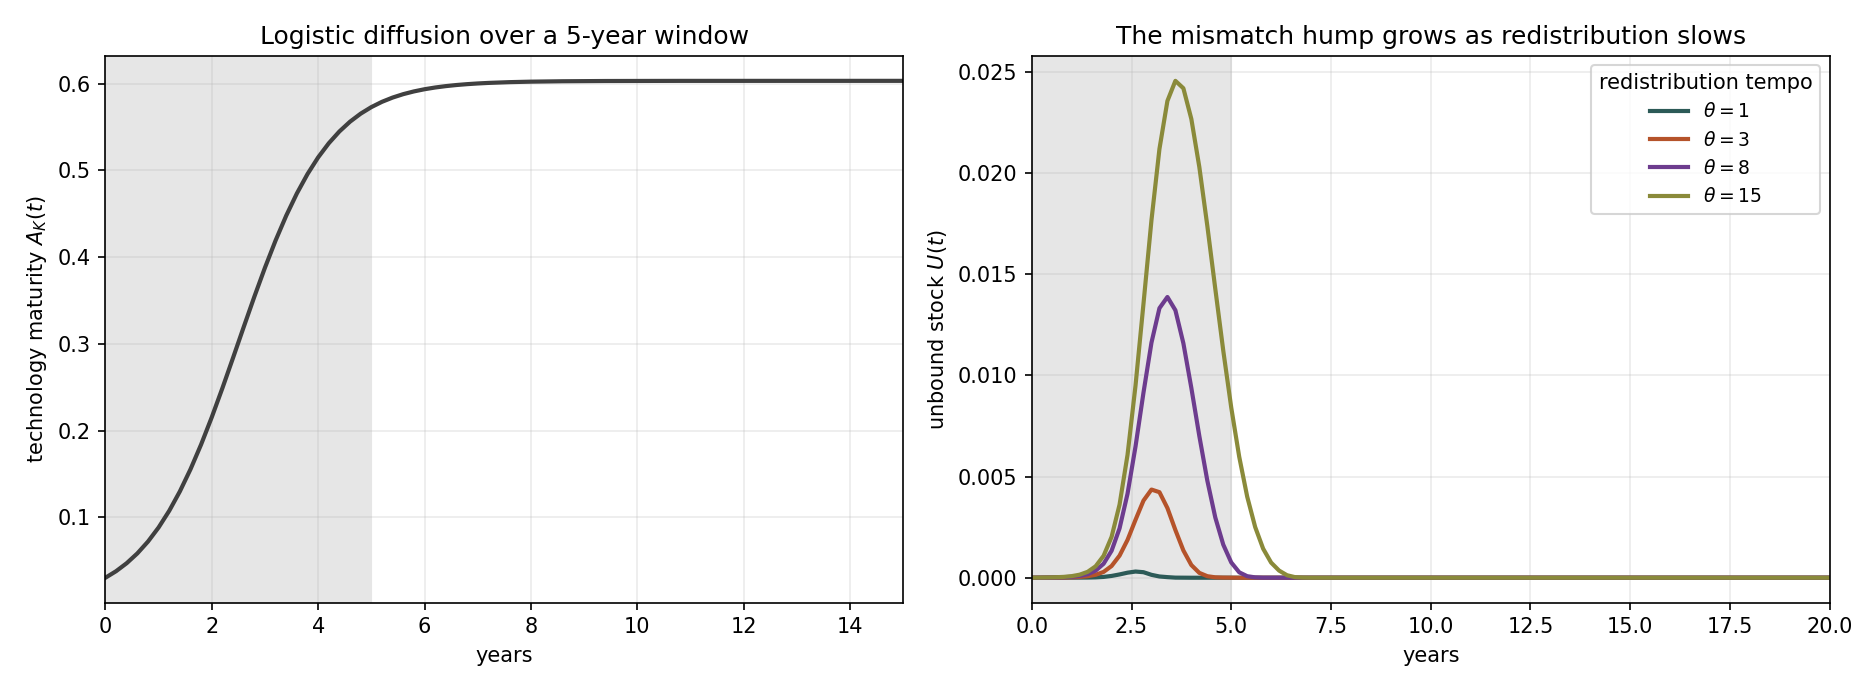
\includegraphics[width=\textwidth]{calendar_dynamics.png}
\caption{Calendar-time dynamics. Left: the technology matures as a
logistic diffusion over a five-year window. Right: the unbound stock
$U(t)$, the transitional mismatch between destruction and creation, for
four redistribution tempos $\theta \in \{1, 3, 8, 15\}$ years against the
fixed five-year shock.
The mismatch hump grows and lingers as redistribution slows relative to
the shock, but always drains to zero: the transitional cost is in the
path, not the endpoint.}
\label{fig:calendar}
\end{figure}

\subsection{The destination depends on the tempo}
\label{sec:destination}

The hump measures the cost of the transition; the same ratio also
determines its outcome. Figure~\ref{fig:tempo} shows where the reinstated
work is bound in two regimes, run through the same technology and the
same field. In the gradual regime ($\theta = 1$ year against the five-year
shock), the best-matched occupations keep pace and absorb the work: the
gainers are the high-skill specialists whose capabilities sit at the
frontier of the field. In the congested regime ($\theta = 15$ years),
the small best-matched occupations cannot bind
fast enough --- their size-limited capacity $c_o = M_o/\theta$ is small,
the mass accumulates in $U$, and it is taken instead by the large,
lower-skilled occupations that can absorb it quickly. The same work is
downgraded. Large low-skill service occupations have played the
absorbing role before: \textcite{autor2013} document their growth as
routine work was automated away. The leading gainers make the point concretely: in the
gradual regime they are preventive-medicine physicians, physicists, and
natural-sciences managers; in the congested regime, fast-food and
counter workers, waiters, and dishwashers.

The shift is not marginal. The final allocations of reinstated mass in
the two regimes correlate at $+0.37$ (Pearson, unweighted across the
$849$ pre-existing occupations; $+0.31$ by rank): substantially different
destinations from one technology and one field, differing only in the
tempo of the shock relative to the market's capacity to respond.
Weighting by baseline employment raises the correlation to $+0.68$,
because the largest occupations gain in both regimes; the divergence is
concentrated in whether specialist best matches or large absorbers take
the frontier work, which is the margin the result is about. This is
the destination counterpart of the transitional hump. The fixed point
sees the endpoint of a frictionless reallocation; the endpoint the
economy actually reaches depends on how fast it was forced to move.

\begin{figure}[t]
\centering

\includegraphics[width=\textwidth]{tempo_regimes.png}
\caption{The destination of reinstated work depends on the tempo ratio.
Both panels show the reinstated task mass gained by each occupation, over
the survival-gated seeding field (grey) with the technology field dashed,
for the same five-year shock. Left, a gradual transition: the best
matches keep pace and high-skill specialists at the frontier absorb the
work. Right, a congested transition: small best-matched occupations
cannot keep up and the work is forced onto large, lower-skilled
occupations. The two final allocations correlate at $+0.37$.}
\label{fig:tempo}
\end{figure}

The mechanism reads off the per-occupation evidence. Define an
occupation's unconstrained claim as the seed-weighted share the claim law
\eqref{eq:claim} would allocate with no size cap, and its size as the
pre-shock task mass that caps the rate. In the gradual regime absorption
tracks the claim --- Pearson $+0.83$, rank $+0.92$ --- and is
uncorrelated with size ($+0.04$); the top claim quartile takes $49$
percent of the reinstated mass. In the congested regime the claim
decouples ($+0.37$, rank $+0.21$) and size takes over (rank $+0.95$);
the top size quartile takes $57$ percent of the mass and the bottom
quartile is squeezed from $22$ to $4$ percent. All rankings are in
absolute mass; the relative-change measure is unbounded for small
occupations and is not used.

Three robustness checks bound the claim. Sweeping the sharpness $\beta_m$
from $1$ to $8$ moves the cross-regime correlation from $+0.26$ to
$+0.61$: the divergence of destinations survives the full range, while
its point size depends on the handle. And decomposing the tempo into its
two timescales shows which one binds: slowing only absorption
($\theta_L = 1$, $\theta_{\text{abs}} = 15$) reproduces the congested
allocation (correlation $+0.39$ with the gradual run), while slowing
only mobility ($\theta_L = 15$, $\theta_{\text{abs}} = 1$) leaves the
destination essentially unchanged ($+1.00$). The forced downgrading is a
statement about how fast occupations can take on new work, not about how
fast workers move.

The third check varies the survival gate itself, since the low-priced
character of surviving seed is inherited from it. Both regimes are rerun
with the gate off, and with a comparative-advantage gate: a
human-productivity field $h(\rr) = \exp[\lambda_h(1-\hat\phi_K(\rr))]$,
with $\hat\phi_K$ the unit-amplitude technology shape, so labour is more
productive where the machine is weak and capital operates where
$s_K\phi_K > h R/\Pi$; $\lambda_h$ is swept up to $2$, and
$\lambda_h = 0$ recovers the uniform-$R$ gate. The divergence is intact
in every variant --- the cross-regime correlation stays between $+0.35$
and $+0.46$, and the congested size rank correlation between $+0.91$ and
$+0.96$. What the gate moves is the gainers' price level, not the tempo
dependence: without the gate the capital-dominated core seeds, and the
congested absorbers become large health and administrative occupations
rather than food service; the comparative-advantage gate raises the
mass-weighted gainer price with $\lambda_h$. The downgrading ---
congested gainers priced below gradual gainers --- persists throughout.

\subsection{The homotopy between the limits}
\label{sec:homotopy}

The tempo result is the path between the two proved endpoints of
Section~\ref{sec:limits}. Figure~\ref{fig:homotopy} traces the final
allocation across $\theta_{\text{abs}}$ from $0.5$ to $120$ years against
the fixed five-year shock, with mobility held fast ($\theta_L = 1$; the
decomposition above shows the destination is carried by
$\theta_{\text{abs}}$). Its correlation with the fast-limit allocation of
Proposition~\ref{prop:fast} falls monotonically from $+1.00$ to $+0.07$,
and its correlation with the size shares of
Proposition~\ref{prop:slow} rises monotonically from $+0.03$ to $+0.94$
($+0.996$ by rank) over the same sweep. The crossover, where the two
associations are equal, sits between $\theta_{\text{abs}} = 10$ and
$15$: two to three shock windows. The simulation's remaining role is to
locate the crossover; the two endpoint allocations are derived.

\begin{figure}[t]
\centering
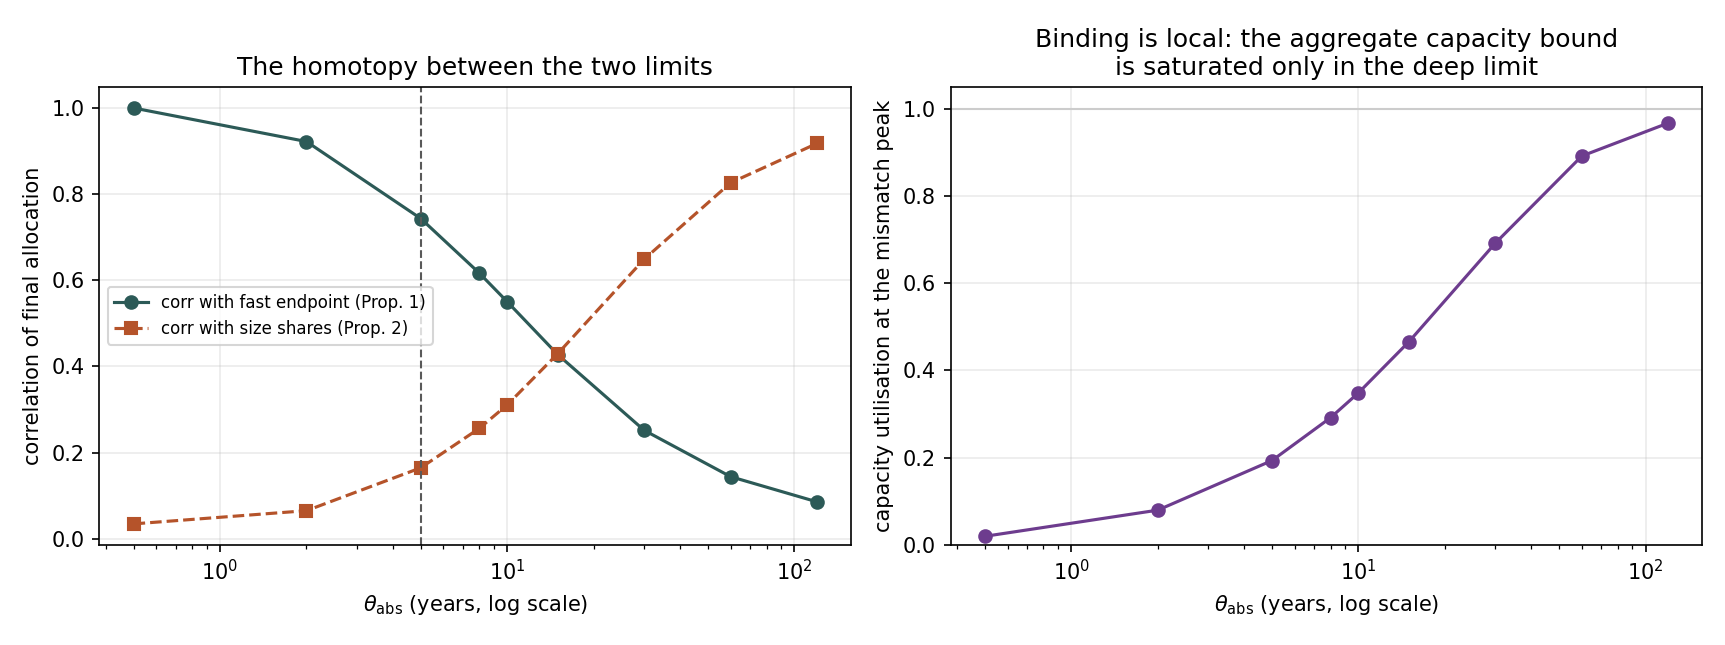
\includegraphics[width=\textwidth]{limit_allocations.png}
\caption{The destination as a homotopy between proved limits. Left: the
correlation of the final allocation with the fast-limit claim allocation
(Proposition~\ref{prop:fast}) and with the slow-limit size shares
(Proposition~\ref{prop:slow}), across the absorption tempo at fixed
mobility; the vertical line marks the shock window. Right: the capacity
utilisation at the mismatch peak, the mass absorbed per step over the
aggregate bound; the shortfall at intermediate tempos is the spatial
locality of binding, and Proposition~\ref{prop:slow} is the regime where
it reaches one.}
\label{fig:homotopy}
\end{figure}

\section{The general-equilibrium price feedback}
\label{sec:ge-feedback}

Both the static regime and the dynamic transition above hold the price field
$\Pi(r)$ fixed: the shock relocates labour and re-sorts it, congestion adjusts
the marginal value of crowded destinations, but the per-unit price of capability
content does not re-solve. This is a short-run reading. The price field is an
equilibrium object, derived as a capability assignment in
\textcite{storck2026fields}, Section~3.3; holding it fixed discards
part of the model's own content. \textcite{acemoglu2024rents} make the point sharply: in their
task model the base wage \emph{adjusts} to automation (their propagation matrix
$\Theta$), and that adjustment is the mechanism. Our fixed-price layers hold even
more fixed than they do --- both the rent wedge and the base price --- so to
``derive the prices'' in their sense we must let the base price move. This
section closes that loop.

\paragraph{The closure: level from data, change from the assignment.}
We keep the level from the estimated field --- the empirical anchor --- and take
the \emph{change} from the assignment, exactly as \textcite{acemoglu2024rents}
take the wage level as given and compute its response. Their wage law
$w_g \propto (\Gamma_g/\ell_g)^{1/\lambda}$ ties the wage to tasks per worker;
its spatial form is
\begin{equation}
  \Delta \ln \Pi(r) \;=\; \frac{1}{\sigma}\Big[\,\ln\big(1-a(r)\big) \;-\; \ln\frac{n_L(r)}{n_L^0(r)}\,\Big],
  \label{eq:price-feedback}
\end{equation}
applied to the baseline, $\Pi(r) = \Pi_0(r)\,e^{\Delta\ln\Pi(r)}$. Automation is a
\emph{demand} shock to labour: where capital takes the task ($a$ high), the task
leaves the human set and the wage falls; and displaced labour crowding the
remaining work ($n_L > n_L^0$) lowers it further. Both terms are stabilising. The
sign is not innocuous: the opposite reading --- treating automation as a
\emph{supply} shock that makes scarce human work dearer --- inverts
equation~\eqref{eq:price-feedback} and is destabilising, since a dearer wage
opens the takeover gate. Run as a single pass at $\sigma = 3$, the scarcity
reading collapses the labour share to $0.33$ (capital chases the work it has just
made dear), while the demand reading lifts it to $0.83$; the fixed-price value
$0.58$ sits between. Labour shares in this section hold the allocation at
its baseline, which isolates the price channel; the headline shares of
\textcite{storck2026fields} re-solve the allocation as well and are correspondingly
higher --- $0.626$ at fixed prices, $0.78$ at the fixed point below. The
headline depends on the sign, which therefore must
be chosen on economic grounds. \textcite{acemoglu2024rents} choose ours:
automation dissipates rents and lowers wages.

\paragraph{The static fixed point.}
Iterating price and allocation to mutual consistency converges, and the
convergence follows from a condition that can be evaluated at the
calibration. Differentiating the gate~\eqref{eq:operated} gives
$\partial \ln(1-a)/\partial \ln\Pi = -a\,(R/\Pi)/\tau$: a lower price
closes the gate, which raises the price back. The slope of the
map~\eqref{eq:price-feedback} is therefore bounded by
\begin{equation}
K \;\le\; \frac{1}{\sigma}\Bigl(\,\sup_{\rr}\,
\frac{a(\rr)\,R}{\Pi(\rr)\,\tau} \;+\; \varepsilon_n\Bigr),
\label{eq:contraction}
\end{equation}
where $\varepsilon_n$ is the crowding elasticity of the re-sorted
density, and damped iteration with weight $d$ converges when the
stabilising slope satisfies $K < 2/d - 1$; at $d = \tfrac12$ the
threshold is $3$. Evaluated at the converged point, the gate term peaks
at $1.64$ and the spectral radius of the full map, crowding included, is
$1.59$ by power iteration: the condition holds with a factor-two margin,
and the iteration converges in nine damped steps. The slope scales as
$1/\sigma$ ($\sigma K = 4.77$ at $\sigma = 0.5$ against $4.78$ at
$\sigma = 3$), which places the failure boundary at $d = \tfrac12$ near
$\sigma = 1.6$; at $\sigma = 1$ the iteration indeed fails at
$d = \tfrac12$ and converges at $d = \tfrac14$. The fixed point itself
does not depend on the damping; only the path to it does.

The self-consistent state
is an interior point, not the one-pass extreme: the labour share settles at
$0.73$ (against $0.58$ at fixed prices), the price level falls $26$ percent, and
displacement is cut by roughly $44$ percent ($D_o$ from $0.28$ to $0.16$). The
wage adjustment absorbs most of the shock: human work becomes about a quarter
cheaper, capital adopts far less, and the labour share stays high --- but the
harm now sits in the wage \emph{level}, not in employment, which is the
rent- and wage-dissipation of \textcite{acemoglu2024rents}.

\paragraph{The dynamic close, and statics meeting dynamics.}
Wired into the transition --- the price responding to the current adoption and
allocation at every step, equation~\eqref{eq:price-feedback} with a one-step lag
--- the feedback shapes the whole path. The wage level falls
monotonically as adoption rises, from $-0.09$ early to a plateau at $-0.29$, and
the displacement wave is markedly gentler: the unbound-mass (mismatch) peak is
cut by about $63$ percent (from $0.44$ to $0.16$ percent of the workforce) at the
same timing, and the reinstated stock ends lower, because the falling wage deters
the automation that would have produced the mismatch. The transition
lands where the static fixed point says it should: the dynamic end-state price
level ($-0.285$) and labour share ($0.739$) reproduce the static fixed point
($-0.26$, $0.73$) to within rounding. Two independent constructions --- static
fixed-point iteration and dynamic time-stepping --- reach the same equilibrium,
so the price feedback is a property of the model rather than of either method,
and the static and dynamic accounts cohere.

\paragraph{What this does and does not establish.}
The feedback is first-order: at fixed prices both layers overstate the
displacement and understate the labour share, and they overstate the violence of
the transition. The stabilising wage adjustment is the shock absorber, and it
operates throughout the transition. The quantitative point
estimate depends on the assignment elasticity $\sigma$ and on the reduced-form
closure --- equation~\eqref{eq:price-feedback} is the AR wage law applied
region-wise, not a full re-solve of the assignment programme of
\textcite{storck2026fields} --- and the AI field remains one illustrative
instance of a technology field, not a measurement. Across $\sigma$ from
$5$ to $0.5$ the fixed-point lift of the labour share runs from $+0.11$
to a peak of $+0.20$ at $\sigma = 1$, and the damping of the mismatch
hump rises from $46$ to $89$ per cent. We therefore read the result
as establishing the \emph{direction and order of magnitude} of the price
feedback, and the mutual consistency of the static and dynamic closes, rather
than a calibrated forecast of the labour share.

%% ============================================================
\section{Discussion}
\label{sec:discussion}
%% ============================================================

The result is that the tempo of a technology shock, relative to the
speed at which the labour market reallocates, determines where the
reinstated work ends up. A gradual diffusion lets work find the
occupations whose capabilities match it; a shock that outruns adjustment
forces a downgrading that persists in the final allocation. The same
field and the same seeded reinstatement yield different allocations of
work depending on the pace. The task-based equilibrium framework is not
built to make this statement: its rest point is the destination of a
frictionless economy, and the friction here is time itself.

Two qualifications bound the claim, and both are inherited rather than
introduced. The first concerns the survival gate. The static model
places surviving reinstatement on the low-priced side of the boundary,
because a seeded task is retained by labour where labour is the cheaper
producer at a \emph{uniform} cost $R$; in
\textcite{acemoglu2019automation} reinstatement is instead new
\emph{complex} work in which labour has a comparative advantage, which
requires the survival condition to turn on relative rather than absolute
productivity. Section~\ref{sec:destination} runs exactly this variant,
alongside the gate removed altogether, and the gate turns out to govern
the \emph{character} of the destination rather than its tempo
dependence: the divergence and the size mechanism survive every variant,
while the gainers' price level moves with the gate. What remains
conditional on the survival-gate economics is therefore the high- versus
low-skill reading of the congested absorbers --- food service under the
absolute gate, large health and administrative occupations without it
--- not the result that a fast shock forces the work onto whoever is
large enough to take it.

The second qualification is the binding calibration. The allocation
depends on the sharpness $\beta_m$ and the absorption timescale
$\theta_{\text{abs}}$, and Section~\ref{sec:destination} reports both
sensitivities: the divergence of destinations survives the sharpness
sweep with a point size that moves with the handle, and it is carried by
the absorption timescale alone. The remaining quantitative claim is the
regime boundary --- how slow absorption must be, relative to the shock,
for downgrading to set in --- which the tempo sweep exhibits rather than
derives.

Several limitations remain. The realisation is illustrative, inheriting
the calibration and discipline of \textcite{storck2026fields}: no
causal claim is made from it. The unbound stock drains to zero, so the model has no
permanent mismatch and no involuntary non-employment; the transitional
cost is the hump, and a model with task decay or irreversible binding
would carry a permanent imprint of the shock speed that this one does
not. The imprint is empirically real and uneven:
\textcite{edin2023individual} find moderate mean earnings losses from
occupational decline, concentrated on low earners. That extension is
left for later work. New tasks enter as added
weight on existing locations rather than as
new points on the disk. And the relative-change measure of who gains is
unbounded for small occupations, so the destination results should be
read in absolute and spatial terms.

The downgrading of the fast regime has an empirical silhouette.
\textcite{beaudry2016great} document a cascade after 2000: as demand for
cognitive tasks fell, high-educated workers moved down the occupational
ladder and pushed the less educated further down and out. The direction
is reversed here. In their account workers descend the ladder because
demand for their tasks has fallen; in the fast regime the work itself
descends the match ranking because the occupations that fit it best are
too small to absorb it in time. The same outward pattern --- work
performed below the skill level that matches it --- arises from
different mechanisms, one demand-side, one absorption-side, and the
cascading image is theirs.

%% ============================================================
\section{Conclusion}
\label{sec:conclusion}
%% ============================================================

Turning the spatial task-based model from an equilibrium into laws of
motion requires one new object, a stock of unbound task mass, and yields
two things the equilibrium cannot. The first is the transitional
mismatch $U(t)$, the gap between destruction and creation as a transient
that grows with the tempo of the shock and drains as the market catches
up. The second, and the central result, is that the tempo of the shock
relative to the speed of redistribution determines the destination of the
reinstated work: a gradual shock matches it to high-skill specialists, a
fast shock forces it onto large lower-skilled occupations. Both
endpoints are proved as limits of the binding law, and the realised
destination moves monotonically between them with the tempo. The same
technology yields a different distribution of work depending only on how
fast it arrives. The cost and the outcome of automation are, in this
sense, properties of the path and not only of the endpoint.

%% ============================================================
\printbibliography
%% ============================================================

\end{document}
